\chapter{ Energy Arbitrage, Imperfect Foresight }
\section{ AEMO Predispatch Forecast Accuracy }
\subsection{ P30 Predispatch Forecast  }
\subsection{ P5 Predispatch Forecast  }
\section{ Methodology }
\section{ Analysis }
\begin{center}
\begin{figure}[!h]
  \caption{FY 2014 - BESS Arbitrage Revenue, Perfect vs. Imperfect Foresight - McConnell (2015)}
  \centering
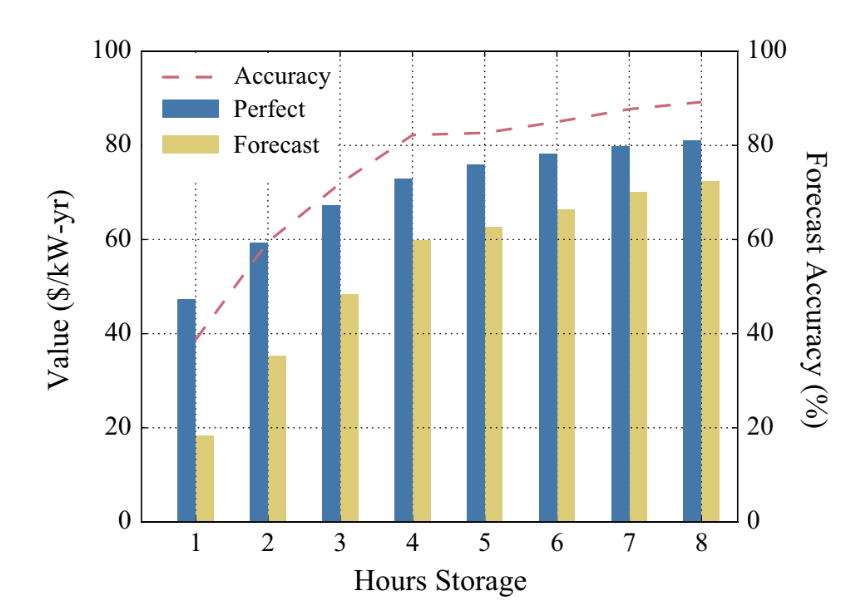
\includegraphics[width=0.8\textwidth]{Pictures/Chapter4/2014_Comp_McCon.png}
\end{figure}
\begin{figure}[!h]
  \caption{FY 2014 - BESS Arbitrage Revenue, Perfect vs. Imperfect Foresight - Blumentals, Tam (2019) }
  \centering
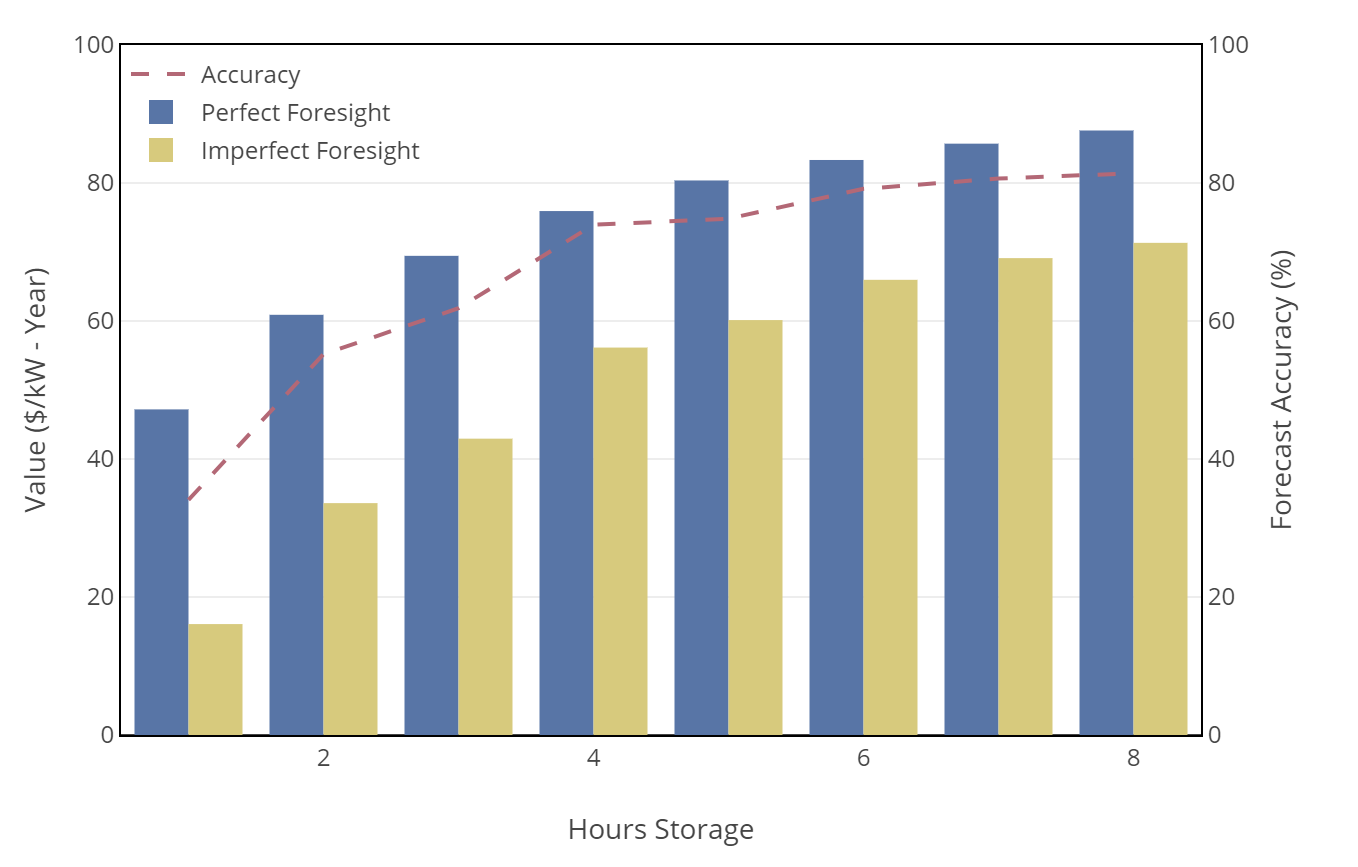
\includegraphics[width=0.8\textwidth]{Pictures/Chapter4/2014_Comp.png}
\end{figure}
\end{center}
\subsection{ Impact of NEM Region, Period and Storage Capacity }
\foreach \x in {NSW,SA,VIC, QLD, TAS}
{ \begin{figure}[!h]
  \caption{\x \; BESS Arbitrage Revenue, Perfect vs. Imperfect Foresight }
  \centering
  \hspace*{-2cm}
\includegraphics[width=1.2\textwidth]{Pictures/Chapter4/\x_Comp.png}
\end{figure}
}

\foreach \x in {NSW,SA,VIC, QLD, TAS}
{ \begin{figure}[!h]
  \caption{\x \; Predispatch Forecast Error }
  \centering
  \hspace*{-2cm}
\includegraphics[width=1.2\textwidth]{Pictures/Chapter4/\x_Predispatch_Accuracy.png}
\end{figure}
}

\subsection{ Impact of P30 Predispatch Accuracy }
\subsection{ Impact of Dynamic Throughput Constraints }
\subsection{ Impact of Applying Bidding Characteristics }